\section{Numerical Simulations}


%%%%%%%%%%%%%%%%%%%%%%%%%%%%%%%%%%%%%%%%%%%%%%%%%%%%%%%%%%%%%%%%
%%%%%%%%%%%%%%%%%%%%%%%%%%%%%%%%%%%%%%%%%%%%%%%%%%%%%%%%%%%%%%%%
%%%%%%%%%%%%%%%%%%%%%%%%%%%%%%%%%%%%%%%%%%%%%%%%%%%%%%%%%%%%%%%%
\subsection{Comparison of Proximal Schemes}

This section compares the following algorithms introduced in Section~\ref{sec-proximal}:
\begin{itemize}
	\item[--] Douglas-Rachford (DR in the following) as exposed in Section~\ref{DR-algo}, parameterized with $\al$ and $\ga$ ;
	\item[--] ADDM on the dual (ADDM in the following, which is DR with $\al=1$) parameterized with~$\ga$ ; 
	\item[--] Primal-dual (PD in the following) as exposed in Section~\ref{PD-algo}, parameterized with~$\si$ and $\tau$.
\end{itemize}
Note that this ADMM formulation is related to the ALG2 method introduced in~\cite{Benamou2000}, but is computed over a staggered grid. For the DR algorithm, we first compared the $4$ possible implementations previously described. It appears in our experiments that A-DR and A-DR' (resp. S-DR and S-DR') have almost the same behavior. 

The first comparison is done on a simple example with two 2-D isotropic Gaussian distributions $(f^0,f^1)$ with the same variance. In the continuous case, the solution is known to be a translation between the mean of the Gaussians. The spatial domain is here of dimension $d=2$ and it is discretized on a grid with $N=M=32$ points for both each dimension. The temporal  discretization has also been fixed to $P=32$. We first compute an (almost) exact reference solution $(m^\star,f^\star)$ of the discrete problem with $10^6$ iterations of the DR. The obtained transported mass $f^\star(\cdot,t)$ is illustrated in Figure \ref{fig:data_bump}. Regarding the computation time, with a bi-processor system Intel Core i7 with 2.4 GHz, $1000$ iterations are done in $45$ seconds for a $32^3$ domain with our Matlab implementation.

\begin{figure}[!ht]
\begin{center}
\begin{tabular}{ccccc}
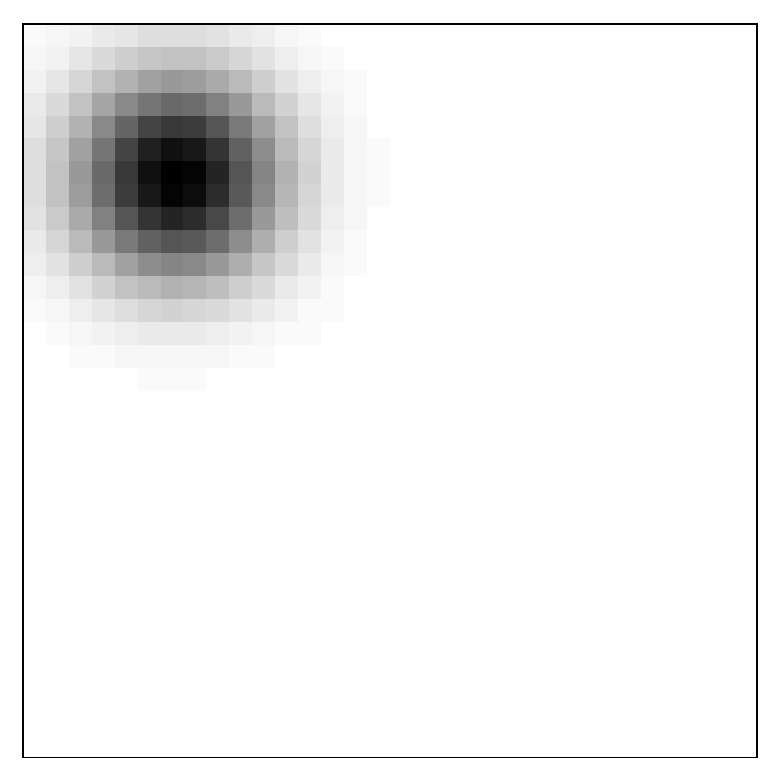
\includegraphics[width=2.5cm]{images/bump_betaold/bump_beta1_01}&
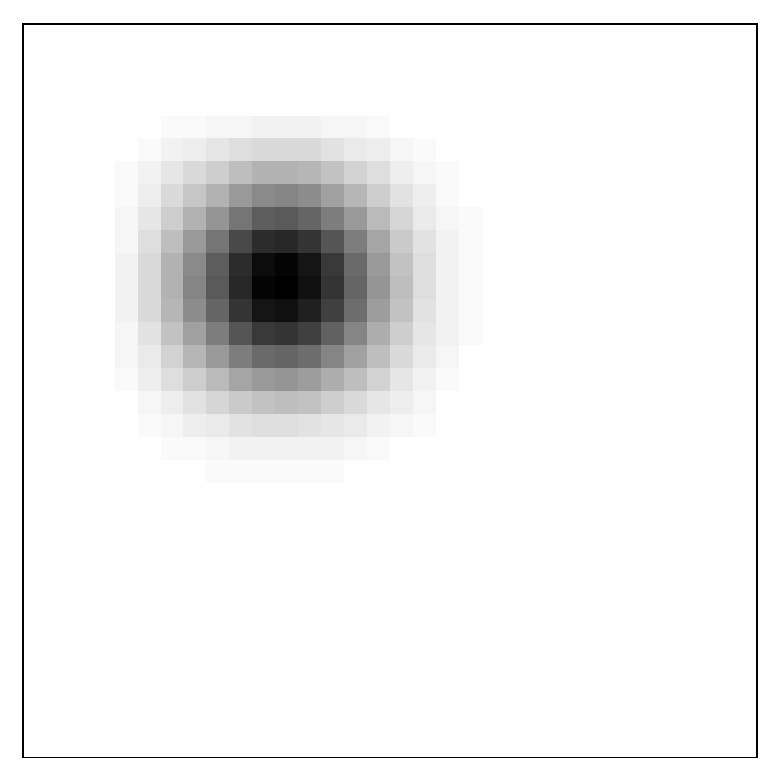
\includegraphics[width=2.5cm]{images/bump_betaold/bump_beta1_09}&
\includegraphics[width=2.5cm]{images/bump_betaold/bump_beta1_17}&
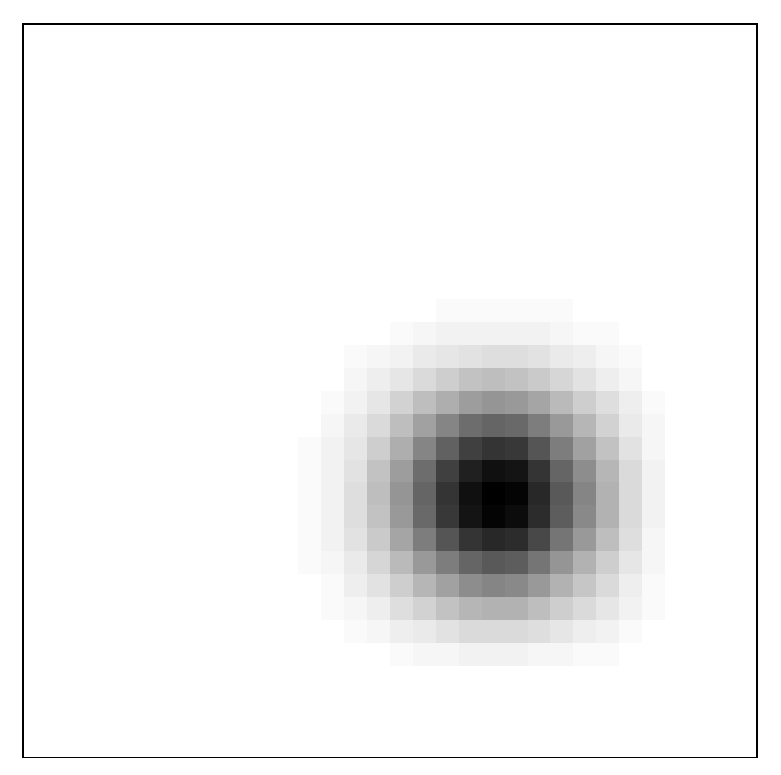
\includegraphics[width=2.5cm]{images/bump_betaold/bump_beta1_25}&
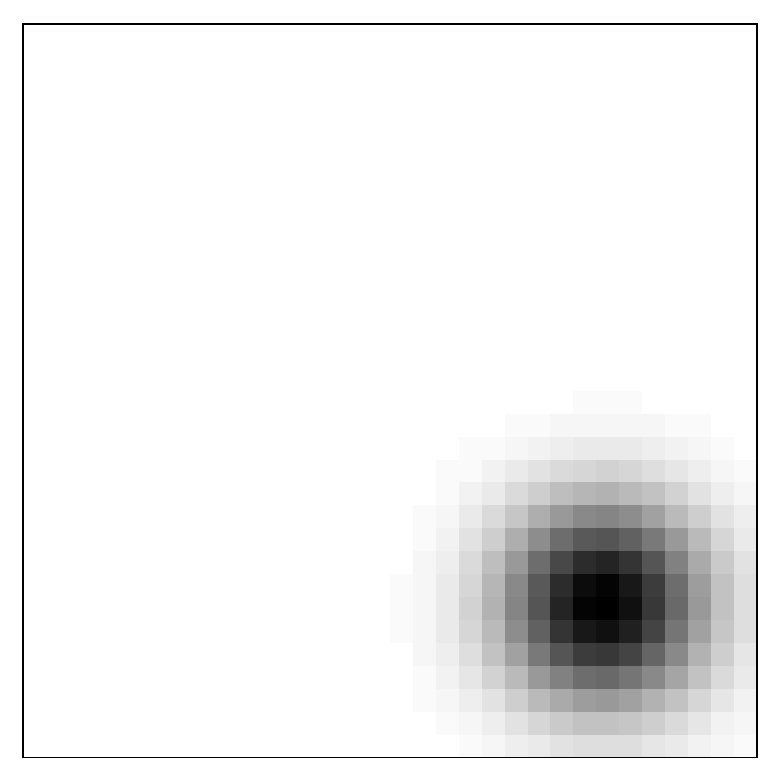
\includegraphics[width=2.5cm]{images/bump_betaold/bump_beta1_33}\\
$t=0$&$t=1/4$&$t=1/2$&$t=3/4$&$t=1$ % \vspace{-0.1cm}
\end{tabular}
\caption{\label{fig:data_bump} 
Display of $f^\star(\cdot,t)$ for several value of $t$ (note that for $t=0$ and $t=1$, this corresponds to $f^0$ and $f^1$). The grayscale values are linearly interpolating from black to white between 0 and the maximum value of $f^\star$. 
}
\end{center}
\vspace{3mm}
\end{figure}

For each algorithm, we perform an exhaustive search of the best possible set of parameters. These optimal parameters are those minimizing $\norm{(m^\star,f^\star) - (\iter{m},\iter{f})}$, the $\ell^2$ distance between $f^\star$ and the output of the algorithm after $\ell=500$ iterations. The optimal parameters for this data set are:  $\ga=1/80$ for ADMM on the dual, $(\ga=1/75,\al=1.998)$ for DR and $\si=85$ for PD. For PD, we found that simply setting $\tau=\frac{0.99}{\si \norm{\interp}^2}$ leads to almost optimal convergence rate in our tests, so we use this rule to only introduce a single parameter $\si$. Notice that this parameter choice is within the range of parameters $\sigma \tau \norm{\interp}^2<1$ that guaranties convergence of the PD method. Figure~\ref{fig:comp_bump} displays, for this optimal choice of parameters, the evolution of the cost function value as well as the  convergence on the staggered grid toward $(m^\star,f^\star)$ as a function of the iteration number $\ell$. 

One can observe that the quality of the approximation can not easily be deduced from the cost function  evolution alone since the functional is very flat. Indeed, an almost minimal value of the function  is reached by all the algorithms after roughly $10^3$ iterations, whereas the $\ell^2$ distance to the reference solution continues to decrease almost linearly in log-log scale. The last plot of the Figure \ref{fig:comp_bump} shows that asymptotically, all methods tend to satisfy the positivity constraint on the staggered grid at the same rate.

\begin{figure}[ht]
\begin{center}
\begin{tabular}{cc}
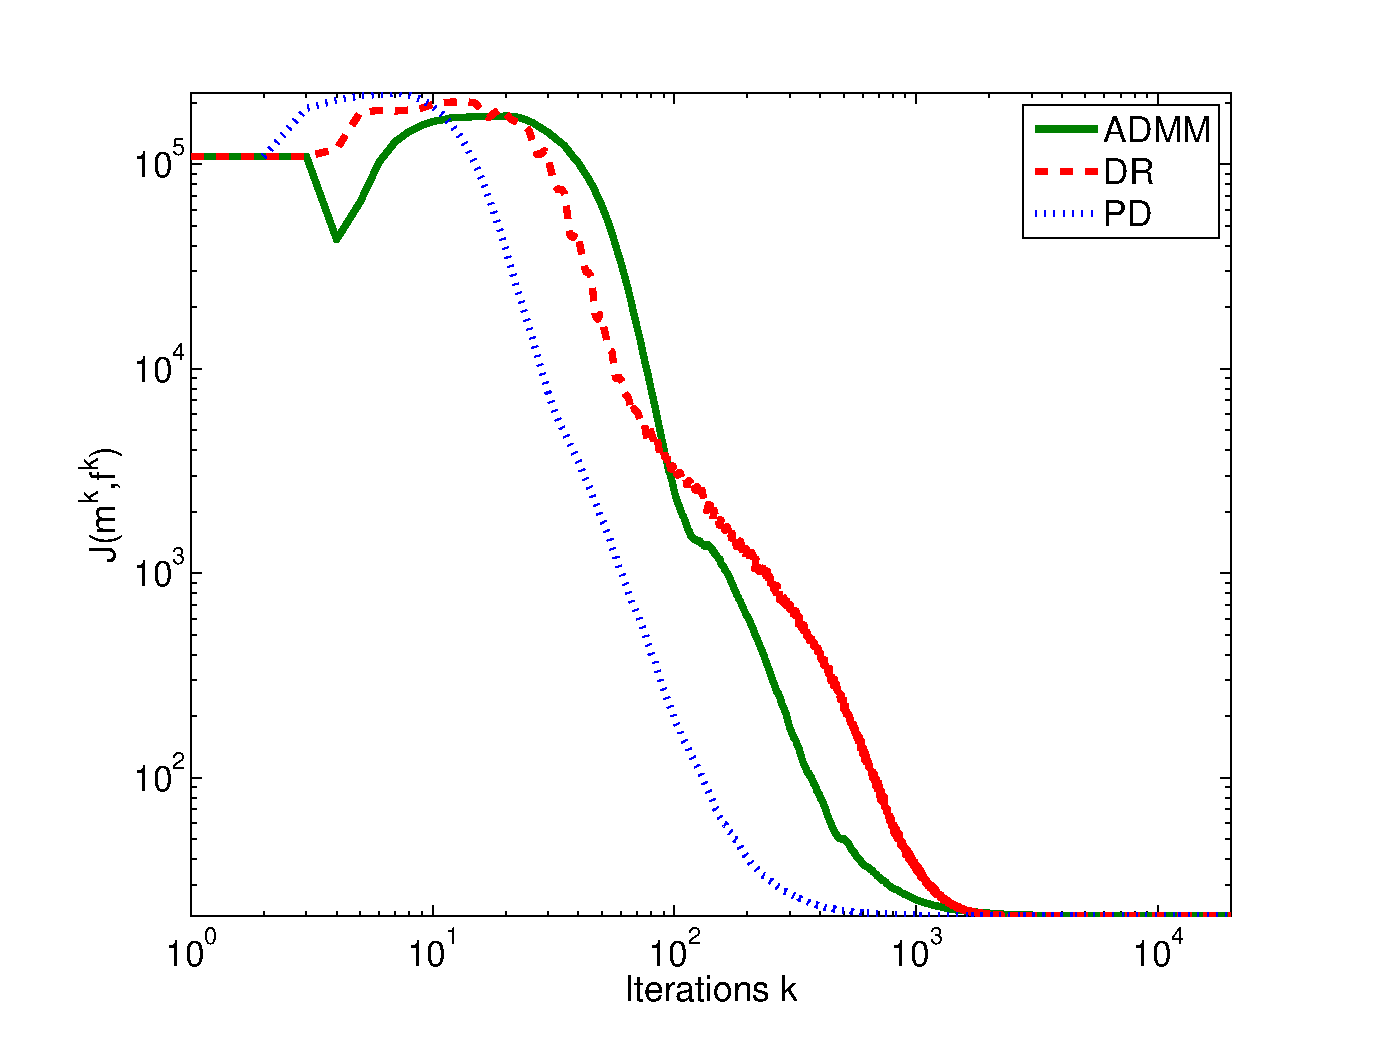
\includegraphics[trim=25 5 45 20,clip,width=0.45\textwidth]{images/J}&\hspace{-0.15cm}
\includegraphics[trim=25 5 45 20,clip,width=0.45\textwidth]{images/M}\vspace{0.1cm}\\
$\Jfunc( \iter{m}, \iter{f} )$&\hspace{-0.15cm}$\norm{m^\star-\iter{m}}$\\
\includegraphics[trim=25 5 45 20,clip,width=0.45\textwidth]{images/F}&\hspace{-0.15cm}
\includegraphics[trim=30 5 45 20,clip,width=0.45\textwidth]{images/Minvalue}\vspace{0.1cm}\\
$ \norm{f^\star-\iter{f}}$ &\hspace{-0.15cm}Mininimum value of $\iter{f}$
\end{tabular}
\caption{\label{fig:comp_bump} 
	At each iteration $\ell$ on the staggered grid, we plot in the log-log scale the value of the cost function $\Jfunc$, the distance between the reference solution $(m^\star,f^\star)$ and the estimation $(\iter{m},\iter{f})$ and the current minimum value of $\iter{f}$ for the different proximal splitting algorithms with the best found parameters. }
\end{center}
\end{figure}

When comparing the three approaches, A-DR and A-PD shows the fastest convergence rate to the reference solution and then, the S-DR algorithm performs equally good as ADMM. This shows the advantage of introducing the $\al$ parameter, while symmetrizing the DR does not speed-up the convergence.  Notice also that the computational cost is smaller for PD, as it takes $0.13$s for one PD iteration and $0.2s$ for one DR or ADMM iteration for this example.  Note that these convergence results are  related to this specific example, but they illustrate the general behaviour of the different algorithms. 

% It can also  be noticed that PD is easier to parameterize. Indeed,  from the necessary relation $\sigma \tau \norm{\interp}^2<1$, one can chose $\si$ and then automatically fix $\tau=\frac{0.99}{\si \norm{\interp}^2}$. The exhaustive search has been realized in this way, thus involving a limited set of possible parameters for PD.

%%%%%%%%%%%%%%%%%%%%%%%%%%%%%%%%%%%%%%%%%%%%%%%%%%%%%%%%%%%%%%%%
%%%%%%%%%%%%%%%%%%%%%%%%%%%%%%%%%%%%%%%%%%%%%%%%%%%%%%%%%%%%%%%%
%%%%%%%%%%%%%%%%%%%%%%%%%%%%%%%%%%%%%%%%%%%%%%%%%%%%%%%%%%%%%%%%

Finally, Figure~\ref{fig:indic} shows an experiment in the context of vanishing and irregular densities.  This figure shows the geodesic, computed with the PD algorithm, between two characteristic functions of two connected sets, one being convex. Note that the geodesic is not composed of characteristic functions of sets, which is to be expected. This shows the ability of our methods to cope with vanishing densities. 



\begin{figure}[!ht]
\begin{center}
\begin{tabular}{@{}c@{}c@{}c@{}c@{}c@{}}
%\animategraphics[palindrome=true,width=3.2cm]{12}{labyrinthe4/bump_obstacle5_iso_}{001}{101}&
\includegraphics[width=2.9cm]{images/shape/shape3_1}&
\includegraphics[width=2.9cm]{images/shape/shape3_17}&
\includegraphics[width=2.9cm]{images/shape/shape3_33}&
\includegraphics[width=2.9cm]{images/shape/shape3_49}&
\includegraphics[width=2.9cm]{images/shape/shape3_65}\\
$t=0$&
$t=1/4$&
$t=1/2$&
$t=3/4$&
$t=1$
\end{tabular}
\caption{\label{fig:indic} Transport between characteristic functions. Evolution of $f^\star(\cdot,t)$ for several values of $t$. The red curve denotes the boundary the area with positive density. }
\end{center}
\end{figure}


%%%%%%%%%%%%%%%%%%%%%%%%%%%%%%%%%%%%%%%%%%%%%%%%%%%%%%%%%%%%%%%%
%%%%%%%%%%%%%%%%%%%%%%%%%%%%%%%%%%%%%%%%%%%%%%%%%%%%%%%%%%%%%%%%
%%%%%%%%%%%%%%%%%%%%%%%%%%%%%%%%%%%%%%%%%%%%%%%%%%%%%%%%%%%%%%%%
\subsection{Interpolation Between $L^2$-Wasserstein and $H^{-1}$}


We first apply the PD algorithm for different values of $\beta$ on the bump example introduced in the previous section. The results are presented in the Figure~\ref{fig:generalized_bump}, which shows the level-lines of the estimated densities $\iter{f}(\cdot,t)$ for $\ell=1000$ iterations. It shows the evolution of the solution between a linear interpolation of the densities ($\beta=0$) and a displacement interpolation with transport ($\beta=1$). 


\newcommand{\sidecap}[1]{ {\begin{sideways}\parbox{1.4cm}{\centering #1}\end{sideways}} }
\newcommand{\myfigBeta}[1]{\includegraphics[width=.105\linewidth]{images/bump_beta/bump_beta_#1}}

\begin{figure}[!ht]
\begin{center}
\begin{tabular}{@{}c@{}c@{}c@{}c@{}c@{}c@{}c@{}c@{}c@{}c@{}}
\sidecap{$\beta=0$ } &
\myfigBeta{0_iso_01}&
\myfigBeta{0_iso_05}&
\myfigBeta{0_iso_09}&
\myfigBeta{0_iso_13}&
\myfigBeta{0_iso_17}&
\myfigBeta{0_iso_21}&
\myfigBeta{0_iso_25}&
\myfigBeta{0_iso_29}&
\myfigBeta{0_iso_33}\\
\sidecap{$\beta=1/4$ } &
\myfigBeta{25_iso_01}&
\myfigBeta{25_iso_05}&
\myfigBeta{25_iso_09}&
\myfigBeta{25_iso_13}&
\myfigBeta{25_iso_17}&
\myfigBeta{25_iso_21}&
\myfigBeta{25_iso_25}&
\myfigBeta{25_iso_29}&
\myfigBeta{25_iso_33}\\
\sidecap{$\beta=1/2$ } &
\myfigBeta{50_iso_01}&
\myfigBeta{50_iso_05}&
\myfigBeta{50_iso_09}&
\myfigBeta{50_iso_13}&
\myfigBeta{50_iso_17}&
\myfigBeta{50_iso_21}&
\myfigBeta{50_iso_25}&
\myfigBeta{50_iso_29}&
\myfigBeta{50_iso_33}\\
\sidecap{$\beta=3/4$ } &
\myfigBeta{75_iso_01}&
\myfigBeta{75_iso_05}&
\myfigBeta{75_iso_09}&
\myfigBeta{75_iso_13}&
\myfigBeta{75_iso_17}&
\myfigBeta{75_iso_21}&
\myfigBeta{75_iso_25}&
\myfigBeta{75_iso_29}&
\myfigBeta{75_iso_33}\\
\sidecap{$\beta=1$ } &
\myfigBeta{100_iso_01}&
\myfigBeta{100_iso_05}&
\myfigBeta{100_iso_09}&
\myfigBeta{100_iso_13}&
\myfigBeta{100_iso_17}&
\myfigBeta{100_iso_21}&
\myfigBeta{100_iso_25}&
\myfigBeta{100_iso_29}&
\myfigBeta{100_iso_33}\\
&$t=0$&$t=1/8$&
$t=1/4$&$t=3/8$&
$t=1/2$&$t=5/8$&
$t=3/4$&$t=7/8$&$t=1$\vspace{-0.2cm}
\end{tabular}
\caption{\label{fig:generalized_bump} 
Display of the level sets of $\iter{f}(\cdot,t)$ for several value of $t$ and $\be$ (note that for $t=0$ and $t=1$, this corresponds to $f^0$ and $f^1$).}
\end{center}
\end{figure}

Figure~\ref{fig:evol_bump_beta} shows for $\beta = 1/2$ and $\be = 3/4$ the evolution of the cost function with the iterations index $\ell$, together with the convergence of the estimate to the reference solution $(m^\star,f^\star)$ (obtained after $10^5$ iterations of the PD algorithm). We can observe that the behavior of the process with $\beta \in ]0,1[$ is different than the one observed for $\beta=1$ in Figure \ref{fig:comp_bump}. Indeed, we observe a faster convergence of the functional value, which is consistent with the fact that $\Jfunc_\bet$ becomes more and more strongly convex as $\be$ approaches $1/2$ (see \eqref{hessian}). The oscillations come from the Newton's descent that only approximate the computation of $\prox_{\ga J_\bet}$.

\renewcommand{\sidecap}[1]{ {\begin{sideways}\parbox{4cm}{\centering #1}\end{sideways}} }

\begin{figure}[!ht]
\begin{center}
\begin{tabular}{@{}l@{}c@{}c@{}c@{}}
\sidecap{$\beta=0.5$ } &
\includegraphics[trim=30 10 40 20,clip,width=0.31\textwidth]{images/J_05}&
\includegraphics[trim=30 10 40 20,clip,width=0.31\textwidth]{images/M_05}&
\includegraphics[trim=30 10 40 20,clip,width=0.31\textwidth]{images/F_05}\\
\sidecap{$\beta=3/4$ } &
\includegraphics[trim=30 10 40 20,clip,width=0.31\textwidth]{images/J_075}&
\includegraphics[trim=30 10 40 20,clip,width=0.31\textwidth]{images/M_075}&
\includegraphics[trim=30 10 40 20,clip,width=0.31\textwidth]{images/F_075}\vspace{0.1cm}\\
& $\Jfunc_\bet( \iter{m},\iter{f} )$ &  $\norm{m^\star-\iter{m}}$ & 
$\norm{f^\star-\iter{f}}$ 
\end{tabular}
\end{center}
\caption{\label{fig:evol_bump_beta} At each iteration $\ell$, we plot the value of the cost function $\Jfunc_\bet(\iter{m},\iter{f})$ and the distance between the reference solution $(m^\star,f^\star)$ and the estimation $(\iter{m},\iter{f})$. The first (resp. second) row presents the result with $\beta=1/2$ (resp. $\bet=3/4$).}
\end{figure}

As a second example, we show in Figure~\ref{fig:generalized_MK} the different morphings obtained between pictures of Gaspard Monge and Leonid Kantorovich. The grayscale representation scales linearly between black (value of 0) and white (value of 1)  and the dimensions are $N+1=75$, $M+1=100$, $P+1=60$, $M$ being the number of discrete points in the second spatial dimension.

\newcommand{\myfigMonge}[1]{\includegraphics[width=.13\linewidth]{images/MK/MK_beta#1}}

\renewcommand{\sidecap}[1]{ {\begin{sideways}\parbox{1.9cm}{\centering #1}\end{sideways}} }

\begin{figure}[!ht]
\begin{center}
\begin{tabular}{@{}c@{\hspace{1mm}}c@{\hspace{1mm}}c@{\hspace{1mm}}c@{\hspace{1mm}}c@{\hspace{1mm}}c@{\hspace{1mm}}c@{\hspace{1mm}}c@{}}
\sidecap{$\beta=0$ } &
\myfigMonge{0_01}&
\myfigMonge{0_11}&
\myfigMonge{0_21}&
\myfigMonge{0_31}&
\myfigMonge{0_41}&
\myfigMonge{0_51}&
\myfigMonge{0_61}\\
\sidecap{$\beta=0.25$ } &
\myfigMonge{025_01}&
\myfigMonge{025_11}&
\myfigMonge{025_21}&
\myfigMonge{025_31}&
\myfigMonge{025_41}&
\myfigMonge{025_51}&
\myfigMonge{025_61}\\
\sidecap{$\beta=0.5$ } &
\myfigMonge{05_01}&
\myfigMonge{05_11}&
\myfigMonge{05_21}&
\myfigMonge{05_31}&
\myfigMonge{05_41}&
\myfigMonge{05_51}&
\myfigMonge{05_61}\\
\sidecap{$\beta=3/4$ } &
\myfigMonge{075_01}&
\myfigMonge{075_11}&
\myfigMonge{075_21}&
\myfigMonge{075_31}&
\myfigMonge{075_41}&
\myfigMonge{075_51}&
\myfigMonge{075_61}\\
\sidecap{$\beta=1$ } &
\myfigMonge{1_01}&
\myfigMonge{1_11}&
\myfigMonge{1_21}&
\myfigMonge{1_31}&
\myfigMonge{1_41}&
\myfigMonge{1_51}&
\myfigMonge{1_61}\\
&$t=0$ & $t=1/6$ &
$t=1/3$ & $t=1/2$ &
$t=2/3$ & $t=5/6$ & $t=1$
\end{tabular}
\end{center}
\caption{\label{fig:generalized_MK} 
Evolution of $f^\star(\cdot,t)$ for several value of $t$ and $\be$.
 The first and last columns represent the data $f^0$ and $f^1$. The intermediate ones present the reference solution $f^\star(t)$ for successive times $t=i/6$, $i=1\cdots 5$. 
 Each line illustrates $f^\star$ for different values $\beta=j/4$, $j=0\cdots 4$ of the generalized cost function. }
\end{figure}


%%%%%%%%%%%%%%%%%%%%%%%%%%%%%%%%%%%%%%%%%%%%%%%%%%%%%%%%%%%%%%%%
%%%%%%%%%%%%%%%%%%%%%%%%%%%%%%%%%%%%%%%%%%%%%%%%%%%%%%%%%%%%%%%%
%%%%%%%%%%%%%%%%%%%%%%%%%%%%%%%%%%%%%%%%%%%%%%%%%%%%%%%%%%%%%%%%
\subsection{Riemannian Transportation}
\label{subsec-riemanian-examples}

We investigate in this section the approximation of a displacement interpolation for a ground cost being the squared geodesic distance on a Riemannian manifold. This is achieved by solving~\eqref{eq-optim-bb-gen} with $\be=1$ but a non-constant weight map $w$.


We exemplify this setting by considering optimal transport with obstacles, which corresponds to choosing weights $w$ that are infinity on the obstacle $\Oo \subset \RR^d \times \RR$, i.e. 
\eq{
	\foralls k \in \Gc, \quad w_k = 1 + \iota_{\Oo}(x_k,t_k) \in \{1,+\infty\}.
}
Note that the obstacles can be dynamic, i.e. the weight $w$ needs not to be constant in time. 

Figure~\ref{labyrinthe} shows a first example where $\Oo$ is a 2-D ($d=2$) static labyrinth map (the walls of the labyrinth being the obstacles and are displayed in black). We use a $50 \times 50 \times 100$ discretization grid of the space-time domain $[0,1]^3$ and the input measures $(f^0,f^1)$ are Gaussians  with standard deviations equal to $0.04$. For Gaussians with such a small variance, this example shows that the displacement interpolation is located  closely to the geodesic path between the centers of the gaussians.

\newcommand{\myfigLab}[1]{\includegraphics[width=.195\linewidth]{images/labyrinthe/bump_obstacle#1}}

\begin{figure}[!ht]
\begin{center}
\begin{tabular}{@{}c@{}c@{}c@{}c@{}c@{}}
\myfigLab{5_iso_001}&
\myfigLab{5_iso_012}&
\myfigLab{5_iso_023}&
\myfigLab{5_iso_034}&
\myfigLab{5_iso_045}\\
$t=0$&
$t=1/9$&
$t=2/9$&
$t=1/3$&
$t=4/9$\\
\myfigLab{5_iso_056}&
\myfigLab{5_iso_067}&
\myfigLab{5_iso_078}&
\myfigLab{5_iso_089}&
\myfigLab{5_iso_101}\\
$t=5/9$&
$t=2/3$&
$t=7/9$&
$t=8/9$&
$t=1$
\end{tabular}
\caption{\label{labyrinthe} 
Evolution of $f^\star(\cdot,t)$ for several values of $t$, using a Riemannian manifold with weights $w_k$ (constant in time) restricting the densities to lie within a 2-D static labyrinth map.  }
\end{center}
\vspace{3mm}
\end{figure}


Figure~\ref{labyrinthe2} shows a more complicated setting that includes a labyrinth with moving walls: a wall appears at time $t=1/4$ and another one disappears at time $1/2$. The difference with respect to the previous example is the fact that $w$ is now time dependent. This simple modification has a strong impact on the displacement interpolation. Indeed, the speed of propagation of the mean of the density is not constant anymore since the density measure is confined in a small area surrounded by walls for $t \in [1/4,1/2]$.

\newcommand{\myfigLabb}[1]{\includegraphics[width=.195\linewidth]{images/labyrinthe4/bump_obstacle#1}}

\begin{figure}[!ht]
\begin{center}
\begin{tabular}{@{}c@{}c@{}c@{}c@{}c@{}}
\myfigLabb{6_iso_001}&
\myfigLabb{6_iso_012}&
\myfigLabb{6_iso_023}&
\myfigLabb{6_iso_034}&
\myfigLabb{6_iso_045}\\
$t=0$&
$t=1/9$&
$t=2/9$&
$t=1/3$&
$t=4/9$\\
\myfigLabb{6_iso_056}&
\myfigLabb{6_iso_067}&
\myfigLabb{6_iso_078}&
\myfigLabb{6_iso_089}&
\myfigLabb{6_iso_101}\\
$t=5/9$&
$t=2/3$&
$t=7/9$&
$t=8/9$&
$t=1$
\end{tabular}
\caption{\label{labyrinthe2} Evolution of $f^\star(\cdot,t)$ for several values of $t$, using a Riemannian  manifold with weights $w_k$ (evolving in time) restricting the densities to lie within a 2-D dynamic labyrinth map (i.e. with moving walls). }
\end{center}
\vspace{3mm}
\end{figure}

As a last example, we present in Figure~\ref{bretagne} an interpolation result in the context of  oceanography in the presence of coast. We here consider Gaussian mixture data in order to simulate the Sea Surface Temperature that can be observed from satellite. In order to model the influence of the sea ground height, we here considered weights $w$ varying w.r.t the distance to the coast. Denoting as $\Oo$ the area representing the complementary of the sea, we define
\eq{
	\foralls k \in \Gc, \quad w_k = 1 + d(x_k,\partial \Oo) + \iota_{\Oo} \in \{1,+\infty\},
} 
where $d(x,\partial \Oo)$ is the Euclidean distance between a pixel location $x$ and the boundary of $\Oo$. The estimation of such interpolations are of main interest in geophysic forecasting applications where the variables of numerical models are calibrated using external image observations (such as the Sea Surface Temperature). Data assimilation methods used in geophysics look for the best compromise between a model and the observations (see for instance~\cite{Blum2009}) and making use of optimal transportation methods in this context is an open research problem.

\newcommand{\myfigBret}[1]{\includegraphics[width=.195\linewidth]{images/bretagne/bretagne_#1}}

\begin{figure}[!ht]
\begin{center}
\begin{tabular}{@{}c@{\hspace{1mm}}c@{\hspace{1mm}}c@{\hspace{1mm}}c@{\hspace{1mm}}c@{}}
\myfigBret{01a}&
\myfigBret{16}&
\myfigBret{32}&
\myfigBret{48}&
\myfigBret{64}\\
$t=0$&
$t=1/4$&
$t=1/2$&
$t=3/4$&
$t=1$
\end{tabular}
\caption{\label{bretagne} Evolution of $f^\star(\cdot,t)$ for several values of $t$, using a Riemannian  manifold with weights $w_k$ defined from the distance to the boundary of the sea domain (its frontier is displayed in black in the first figure). }
\end{center}
\vspace{3mm}
\end{figure}
